\chapter{Software Architektur}

\section{Logische Sicht}
Das System besteht aus prim"ar 4 Schichten (3  Schichten - Architektur plus Netzwerk). Diese beinhalten:
\begin{description}
\item[Schicht 1] Graphisches User Interface (GUI)
\item[Schicht 2] Problem Domain (PD)
\item[Schicht 3] Datenhaltung (DH)
\item[Schicht 4] Netzwerk (bestehend aus Client und Server)
\end{description}

\begin{figure}[H]
  \begin{center}
    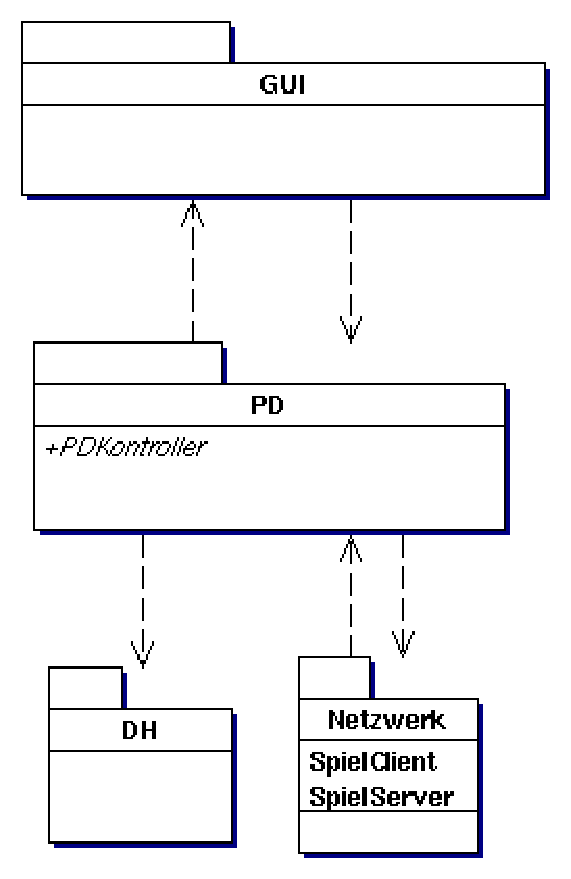
\includegraphics[height=8cm]{./images/architektur.pdf}
  \end{center}
  \caption{Schichtenmodell}
\end{figure}

Diese Architektur haben wir gew"ahlt um eine klare Trennung zwischen den einzelnen Programmteilen zu erreichen. \\
Das graphische User Interface ist die Schnittstelle zum Benutzer. "Uber dieses kann er Eingaben machen oder in unserem Fall erfolgt die Steuerung
der Spielfigur "uber das GUI. \\
Die PD ist die Schicht zwischen GUI und DH. Das heisst sie bekommt und verarbeitet Befehle vom GUI, schreibt Daten in die DH und
ruft Funktionen in der Netzwerkschicht auf. \\
Die Datenhaltung ist daf"ur zust"andig, Daten, die konsistent sein m"ussen zu speichern, damit sie bei einem Neustarten des Spiels wieder
zur Verf"ugung stehen. \\
Die Netzwerkschicht regelt die Daten"ubertragung zwischen dem Server und den Clients.



\section{Netzwerk}

\begin{figure}[hp]
  \begin{center}
    {\rotatebox{90}{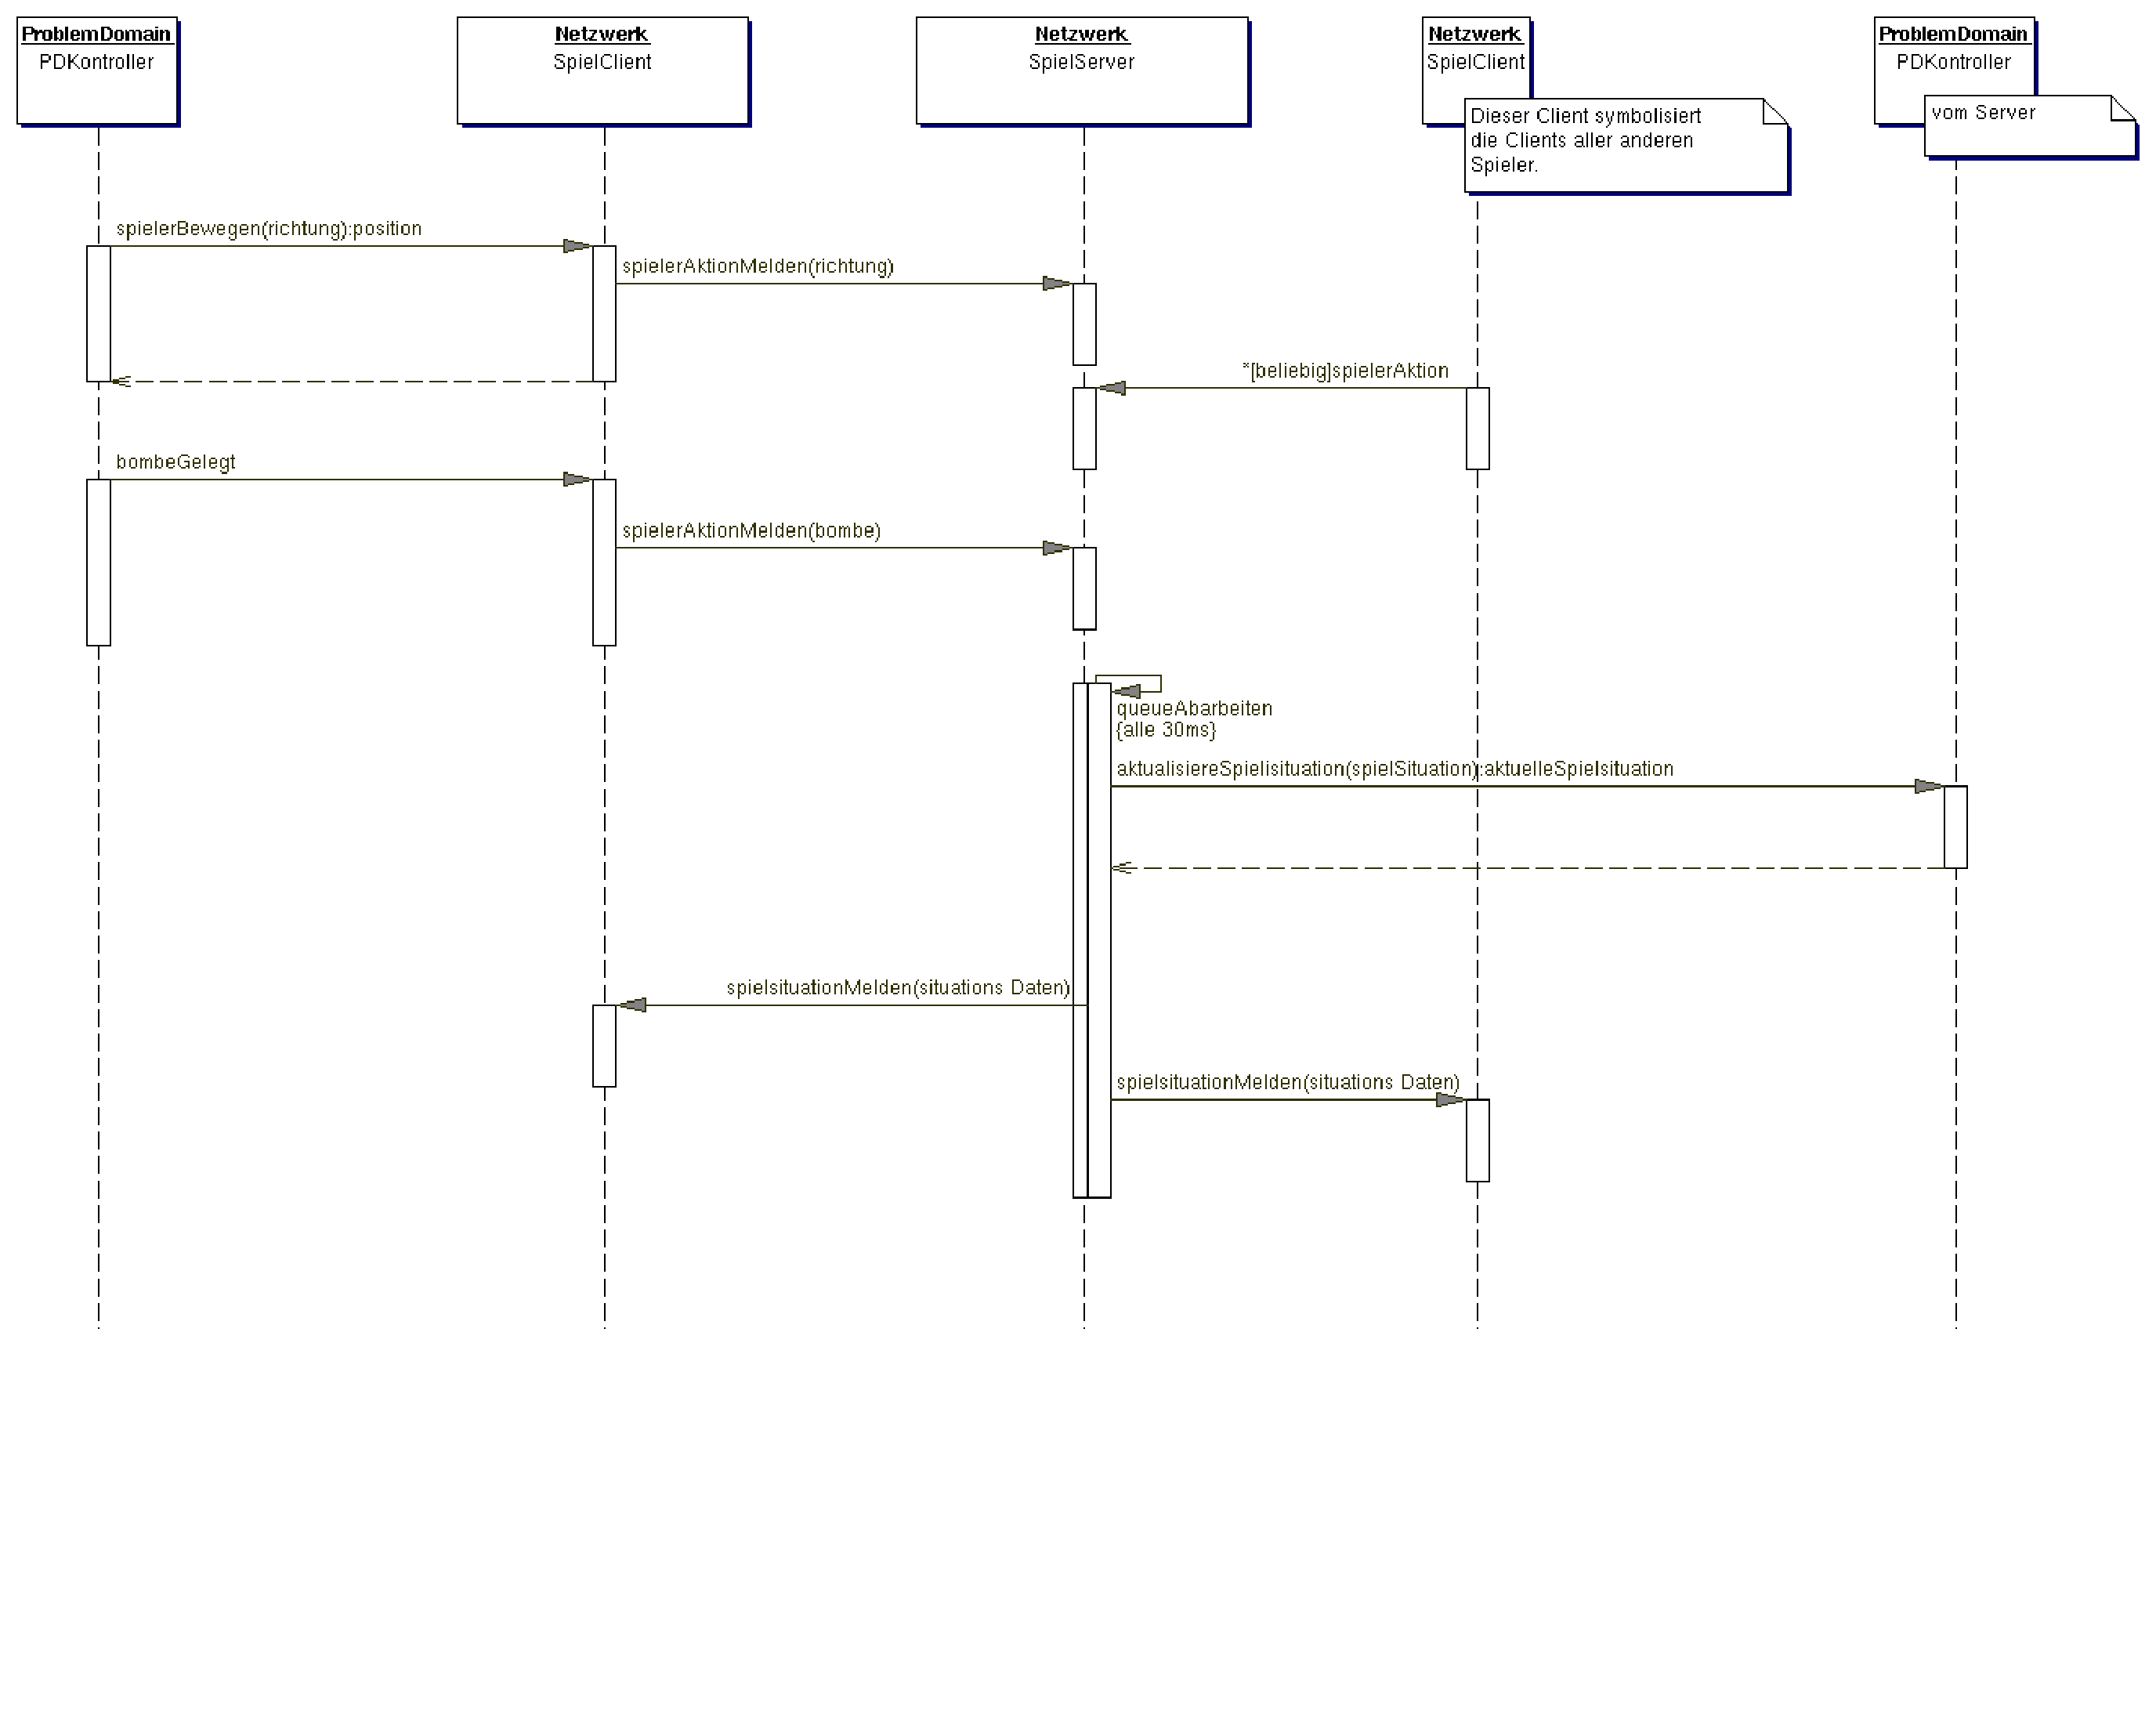
\includegraphics[height=16cm]{./images/netzwerk_aktion.pdf}}}
  \end{center}
  \caption{Interaktionsmodell Netzwerk}
\end{figure}

Das Netzwerk besteht aus einem Server und bis zu vier Clients die miteinander kommunizieren. Dabei kann jeder Client auch Server sein, das heisst
zu Beginn des Spiels entscheidet der Spieler, ob er Server und Client oder nur Client ist. Es kann nur ein Spieler Server sein.
Ist ein Spieler Server und Client, werden die Daten der Mitspieler zu ihm "ubermittelt. Das geschieht folgendermassen: \\
Die aktuellen Bewegungen eines Clients, also eines Spielers, werden zum Server "ubermittelt. Diese Daten werden vom Server
entgegengenommen. Dieser berechnet damit die aktuelle Position und allf"allige Aktionen des Clients. Diese berechnete Postion schickt der Server dann \textit{allen} Clients
zur"uck. Das heisst, jeder Client bekommt vom Server einen Snapshot. Zus"atzlich zur Position beinhaltet dieser wichtige Daten wie zum Beispiel ob
eine Bombe gelegt worden ist oder ein Powerup aufgenommen wurde. Mit diesen Angaben berechnet der Client selbst"andig, was auf dem
Spielfeld passiert. Er macht also dieselben Berechnungen wie der Server. Falls ein Spielelement gel"oscht werden muss,
versucht der Client das zu machen. Da er aber nicht selbst"andig Elemente l"oschen darf, wartet er auf den Befehl des Servers,
das entsprechende Element zu l"oschen. Der Client f"uhrt also nur eine Art Dummy-Funktion aus.
Damit erreichen wir eine bessere Performace wie mit dem Prinzip, bei dem alle Daten vom Server zum Client geschickt werden und zudem
k"onnen wir damit sicherstellen, dass alle Clients den selben Spielstand haben. Die Verbindung l"auft "uber TCP, was das Ankommen
der Pakete sicherstellt. \\
Der Server wurde mit dem Reactor Pattern implementiert. Dieses wird nachfolgend noch genauer erkl"art.
